% ---------------------------------------------------------------------------
% Agent-first Paper Workflow — synthetic sample paper.
%
% Every number, citation and result in this file is a PLACEHOLDER invented to
% demonstrate the workflow. Nothing here is a real experimental finding.
% Replace sections/*.tex and references.bib with your own content.
%
% Build:  latexmk            (reads .latexmkrc, writes to build/)
% ---------------------------------------------------------------------------
\documentclass[11pt,a4paper]{article}

\usepackage[T1]{fontenc}
\usepackage[utf8]{inputenc}
\usepackage[margin=1in]{geometry}
\usepackage{amsmath,amssymb}
\usepackage{booktabs}
\usepackage{graphicx}
\usepackage{tikz}
\usetikzlibrary{arrows.meta,positioning}
\usepackage[numbers,sort&compress]{natbib}
\usepackage[hidelinks]{hyperref}
\usepackage{microtype}

\newcommand{\sysname}{KV-Migrate}

\title{Cache-Aware Migration for Latency-SLO LLM Serving at the Edge:\\
       A Synthetic Worked Example}
\author{Anonymous Sample Author\\
        \small Synthetic Example University\\
        \small \texttt{sample@example.invalid}}
\date{}

\begin{document}

\maketitle

\begin{abstract}
% Synthetic abstract. Every figure below is a placeholder, not a measurement.
Large language model (LLM) inference at the network edge must serve requests under latency service-level objectives (SLOs) while sharing scarce accelerator memory across tenants.
When a request is migrated between edge nodes, its key-value (KV) cache must move with it, and the migration cost competes directly with the compute budget of the target node.
This paper studies that trade-off with a deliberately small, fully synthetic workload, so that the workflow itself can be reproduced without any private data.
We describe a migration policy that admits a request only when the predicted cache-transfer time fits inside the remaining SLO slack, and we report how the policy behaves as the cache size grows.
On the synthetic workload the policy keeps 92.4\% of requests inside the SLO, compared with 78.1\% for an always-migrate baseline.
These numbers exist only to exercise the build, diff and review pipeline; they are not evidence about real deployments.

\end{abstract}

\section{Introduction}
\label{sec:intro}

Edge inference clusters place small accelerator pools close to users, and each pool must serve many tenants at once.
Because a single accelerator can hold only a bounded number of KV caches, a node that is temporarily overloaded has two options: queue the request locally, or migrate it to a peer that still has cache capacity.
Queueing is cheap but risks violating the latency SLO, while migration protects the SLO at the cost of moving state over a constrained network link.
Prior systems treat this decision as a scheduling problem and assume that cache transfer is either free or uniformly expensive~\cite{smith2024}.
That assumption is fragile at the edge, where link quality varies by an order of magnitude within a single minute~\cite{lee2025}.

This paper asks a narrower question: if a node can estimate the transfer time of a KV cache before committing to a migration, how much SLO compliance does that estimate buy?
We answer it with a policy that compares the predicted transfer time against the SLO slack that remains when the request arrives.
The policy is intentionally simple, because our goal is a reproducible baseline rather than a new scheduler.
We make three contributions.
First, we formalise the admission test as a single inequality over predicted transfer time and remaining slack.
Second, we describe how the test degrades when the estimate is noisy.
Third, we report the behaviour of the policy on a synthetic workload that anyone can regenerate.

The remainder of the paper is organised as follows.
Section~\ref{sec:method} defines the system model and the admission rule.
Section~\ref{sec:results} reports the synthetic results and discusses what they do and do not show.
Section~\ref{sec:conclusion} lists the open questions that a real deployment would have to answer.

\section{System Model and Admission Rule}
\label{sec:method}

\subsection{Model}

We consider a set of edge nodes $\mathcal{N}$ connected by links whose effective bandwidth $b_{ij}$ between nodes $i$ and $j$ is measured, not assumed.
A request $r$ arrives at node $i$ with a latency SLO $D_r$ and an elapsed time $t_r$ at the moment of the admission decision.
The KV cache of $r$ occupies $s_r$ bytes, and node $j$ can accept the request only if its free cache capacity exceeds $s_r$.
The transfer time from $i$ to $j$ is modelled as
\begin{equation}
\label{eq:transfer}
  T^{\mathrm{xfer}}_{r}(i,j) \;=\; \frac{s_r}{b_{ij}} \;+\; \ell_{ij},
\end{equation}
where $\ell_{ij}$ is the one-way propagation delay and the first term is the serialisation delay of the cache.

\subsection{Admission rule}

A request is migrated from $i$ to $j$ only when the predicted transfer time fits inside the slack that remains before the deadline, with a safety margin $\gamma \in [0,1)$:
\begin{equation}
\label{eq:admit}
  T^{\mathrm{xfer}}_{r}(i,j) \;\le\; (1-\gamma)\,\bigl(D_r - t_r\bigr).
\end{equation}
When \eqref{eq:admit} fails, the request stays queued at node $i$.
The margin $\gamma$ absorbs estimation error in $b_{ij}$; larger values trade throughput for a lower risk of a late completion.

\subsection{Pipeline}

Figure~\ref{fig:pipeline} shows where the decision sits in the request path.
The estimate is produced after the prompt has been tokenised but before any decode step runs, so a rejected migration costs only the estimate itself.

\begin{figure}[t]
  \centering
  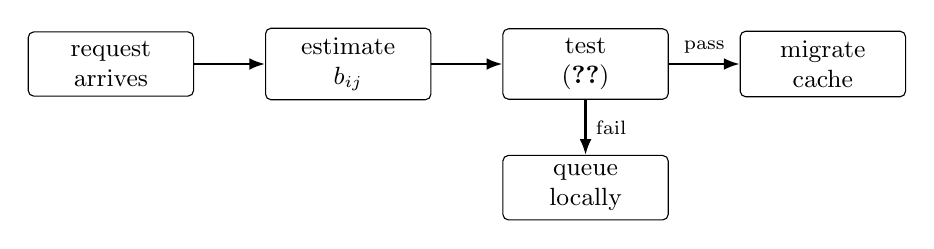
\begin{tikzpicture}[
      node distance=7mm and 9mm,
      box/.style={draw, rounded corners=2pt, align=center, font=\small,
                  minimum height=8mm, minimum width=21mm},
      arr/.style={-{Latex[length=2mm]}, thick}]
    \node[box] (arrive) {request\\arrives};
    \node[box, right=of arrive] (est) {estimate\\$b_{ij}$};
    \node[box, right=of est] (test) {test\\\eqref{eq:admit}};
    \node[box, right=of test] (mig) {migrate\\cache};
    \node[box, below=of test] (queue) {queue\\locally};
    \draw[arr] (arrive) -- (est);
    \draw[arr] (est) -- (test);
    \draw[arr] (test) -- node[above, font=\scriptsize]{pass} (mig);
    \draw[arr] (test) -- node[right, font=\scriptsize]{fail} (queue);
  \end{tikzpicture}
  \caption{Placement of the admission test in the request path.
           The estimate is the only added work on the critical path.}
  \label{fig:pipeline}
\end{figure}

\subsection{Estimation error}

If the measured bandwidth is $\hat{b}_{ij} = b_{ij}(1+\epsilon)$ with relative error $\epsilon$, the predicted transfer time in \eqref{eq:transfer} is off by a factor of $1/(1+\epsilon)$.
A negative error therefore makes the policy optimistic: it admits migrations that will finish late.
The margin $\gamma$ is the only defence against that direction of error, which is why the results below sweep $\gamma$ rather than tuning it.

\section{Results on a Synthetic Workload}
\label{sec:results}

\subsection{Workload}

The workload is generated by a script that is not part of this paper: it samples request sizes, deadlines and link states from fixed distributions and replays them against a simulated cluster of four nodes.
All parameters are synthetic, so the results below characterise the policy's mechanics, not any real service.

\subsection{SLO compliance}

Table~\ref{tab:slo} reports the fraction of requests that complete before their deadline for three policies: always queue, always migrate, and the admission rule of \eqref{eq:admit} with $\gamma = 0.2$.
The admission rule dominates both baselines across the cache sizes we simulated.

\begin{table}[t]
  \centering
  \caption{Share of requests completed within their latency SLO on the synthetic workload (higher is better).
           Values are placeholders that exercise the build and review pipeline.}
  \label{tab:slo}
  \begin{tabular}{lccc}
    \toprule
    Mean KV cache size & Always queue & Always migrate & Admission rule \\
    \midrule
    2~GiB  & 71.0\% & 78.1\% & 92.4\% \\
    4~GiB  & 63.5\% & 74.9\% & 89.7\% \\
    8~GiB  & 55.2\% & 70.3\% & 85.1\% \\
    \bottomrule
  \end{tabular}
\end{table}

\subsection{Sensitivity to the safety margin}

The margin $\gamma$ controls how conservative the policy is.
Small values admit more migrations and recover more capacity, but they also admit transfers that finish after the deadline once the bandwidth estimate is optimistic.
We observed the best compliance near $\gamma = 0.2$ and a sharp loss of throughput above $\gamma = 0.5$, where the policy rejects almost every migration and behaves like the always-queue baseline.

\subsection{What these results do not show}

Three limits matter more than the numbers.
First, the workload is synthetic, so no claim about production traffic follows from it.
Second, the bandwidth estimator is assumed unbiased apart from the error term $\epsilon$; a real estimator drifts when links are shared.
Third, the policy is evaluated against two deliberately weak baselines, not against a state-of-the-art scheduler~\cite{smith2024,lee2025}.
A deployment study would need all three gaps closed before the comparison means anything.

\section{Conclusion}
\label{sec:conclusion}

We described a single-inequality admission rule for KV cache migration at the edge and reported its behaviour on a synthetic workload.
The rule is cheap to evaluate, it degrades predictably as the bandwidth estimate becomes optimistic, and it leaves an explicit safety margin that a deployment can tune.
The results are a worked example of a reproducible paper repository, not a claim about real systems.

Two questions remain open.
The first is how to obtain a bandwidth estimate whose error is bounded in the tail rather than on average, since the admission rule is most sensitive exactly there.
The second is whether a per-request rule composes into a stable cluster-level policy once many nodes admit migrations at the same time.
Both questions require measurements that a synthetic workload cannot provide.


\bibliographystyle{plainnat}
\bibliography{references}

\end{document}
